
%(BEGIN_QUESTION)
% Copyright 2015, Tony R. Kuphaldt, released under the Creative Commons Attribution License (v 1.0)
% This means you may do almost anything with this work of mine, so long as you give me proper credit

Calculate the amount of current output to the ammeter by the current transformer (CT) under normal load conditions, assuming a balanced three-phase source and a balanced three-phase load:

$$\includegraphics[width=15.5cm]{i02881x01.eps}$$

$I_{ammeter}$ = \underbar{\hskip 50pt} A

\vskip 50pt

Now, re-calculate the ammeter's current supposing a tree branch falls across lines A and C, causing a low-resistance fault:

$$\includegraphics[width=15.5cm]{i02881x02.eps}$$

$I_{ammeter}$ = \underbar{\hskip 50pt} A

\vskip 10pt

Hint: you will need to consider phase angles for the fault current calculation!  Feel free to assume an ABC phase rotation, where $V_A = 7200 \hbox{ V } \angle 0^o$ and  $V_B = 7200 \hbox{ V } \angle -120^o$ and $V_C = 7200 \hbox{ V } \angle 120^o$.

\vfil 

\underbar{file i02881}
\eject
%(END_QUESTION)





%(BEGIN_ANSWER)

This is a graded question -- no answers or hints given!
 
%(END_ANSWER)





%(BEGIN_NOTES)

Under normal load conditions, each of the load phases (65 ohms) sees 7200 volts from the source.  Ohm's Law yields the load phase current, which is equal to line current for any Wye network:

$$I_A = {V_A \over R_A} = {7200 \hbox{ V} \angle 0^o \over 65 \> \Omega \angle 0^o} = 110.77 \hbox{ A} \angle 0^o$$

The CT with its 300:5 ratio reduces line current by that factor but (ideally) leaves the phase angle unaltered:

$$I_{ammeter} = 110.77 \hbox{ A} \angle 0^o \div {300 \over 5} = 1.846 \hbox{ A} \angle 0^o$$

\vskip 10pt

The inclusion of a low-resistance fault complicates matters significantly.  First, the fault resistance of 10 ohms is placed across two phases (line A to line C), not between one line and ground as is the case with the 65 ohm load phase resistance.  Not only does this mean the 10 ohm tree branch sees more voltage than any of the phase resistors, but it also sees a voltage {\it at a different phase angle than zero degrees}.

\vskip 10pt

First, calculating the voltage between lines A and C:

$$V_{AC} = V_A - V_C = 7200 \hbox{ V} \angle 0^o - 7200 \hbox{ V} \angle 120^o = 12470.8 \hbox{ V} \angle -30^o$$

Now we may apply Ohm's Law to the calculation of fault current (i.e. current through the fallen tree branch):

$$I_{fault} = {V_{AC} \over R_{fault}} = {12470.8 \hbox{ V} \angle -30^o \over 10 \> \Omega \angle 0^o} = 1247.1 \hbox{ A} \angle -30^o$$

The current passing through the CT will be the sum of this fault current and the normal load current, in accordance with Kirchhoff's Current Law:

$$\includegraphics[width=15.5cm]{i02881x03.eps}$$

$$I_A + I_{fault} = 110.77 \hbox{ A} \angle 0^o + 1247.1 \hbox{ A} \angle -30^o = 1344.15 \hbox{ A} \angle -27.6^o$$

The CT with its 300:5 ratio reduces line current by that factor but (ideally) leaves the phase angle unaltered:

$$I_{ammeter} = 1344.15 \hbox{ A} \angle -27.6^o \div {300 \over 5} = 22.40 \hbox{ A} \angle -27.6^o$$



%INDEX% Electronics review: 3-phase voltage/current/power calculation

%(END_NOTES)


